\section{Fundamentals of \LaTeX I: structure}
\label{sec:struct}

\subsection{Sections}
\label{sec:sec}
The following section type may be used:

\begin{verbatim}
  \section[TitleInTOC]{FullTitle}\label{sec:SectionLabel}
  \subsection[TitleInTOC]{FullTitle}\label{sec:SectionLabel}
  \subsubsection[TitleInTOC]{FullTitle}\label{sec:SectionLabel}
\end{verbatim}
If case you need even more structure depth, you can also use

\begin{verbatim}
  \paragraph{Title}
  \subparagraph{Title}.
\end{verbatim}
However, you cannot reference (sub-)paragraphs. Think about whether you really
need them or if changing the structure might be better. Making it less complex
usually makes it easier to read (and write!).

It is recommended to write special characters like the German \ss, \"a,
\"o, \"u, etc. in \TeX-code without any packages, i.e. \verb!\ss!, \verb!\"a!,
\verb!\"o!, and \verb!\"u!. This in general prevents difficulties if somebody
else is compiling parts of your work who might not use those packages. You
will quickly get used to it!

\subsection{Floats}
\label{sec:float}


\subsubsection{Figures}
\label{sec:fig}

Figures are to be included in the float environment \verb!\figure! as follows

\begin{verbatim}
  \begin{figure}[placement specifier]
    \centering
    \includegraphics[width=0.3\textwidth]{NameOfGraphic}
    \caption{Description of graphic.}
    \label{fig:GraphicLabel}
  \end{figure}.
\end{verbatim}

It is highly recommended to use .eps file format for figures only. You can easily convert almost any given format to .eps using GIMP.\\
\linebreak\\
The size of the graphic (height or width) should be defined relative to the
textheight or -width, respectively. Two figures next to each other are
included by 

\begin{verbatim}
  [...]
  \includegraphics[width=0.3\textwidth]{NameOfGraphic_1}~
  \includegraphics[width=0.3\textwidth]{NameOfGraphic_2}
  [...],
\end{verbatim}
where as figures on top of each other are included by

\begin{verbatim}
  [...]
  \includegraphics[width=0.3\textwidth]{NameOfGraphic_1}\\
  \includegraphics[width=0.3\textwidth]{NameOfGraphic_2}
  [...].
\end{verbatim}

The placement specifier defines where the figure should be placed
\emph{approximately}. This can be \verb!h!, \verb!t!, \verb!b!, or \verb!p!
which stands for \verb!here!, \verb!top of page!, \verb!bottom of page!, or
\verb!own page for floats!. In 90\% of the cases, \LaTeX~knows best where to
put the floats - leave it out. Trying to put the figures exactly where you
want to put them using \verb!h! is a time waster and counts as
procrastination. The history of students - including me - trying to be smarter
than \LaTeX~is as old as \LaTeX~itself - if not older. Nobody succeeded. 
If you do decide to use it after all, try it right before printing the (very, very) final version.

Note that no endings should be set to the graphic's name. Compiling with
\verb!latex! will automatically choose vector graphics with this name, in
contrast to \verb!pdflatex! that will include raster graphics. Let
\LaTeX~choose the appropriate format - just make sure that you provide a
graphic of an appropriate format in the given graphic path (see "Lead up" in
header file).

\begin{figure}[placement specifier]
  \centering
  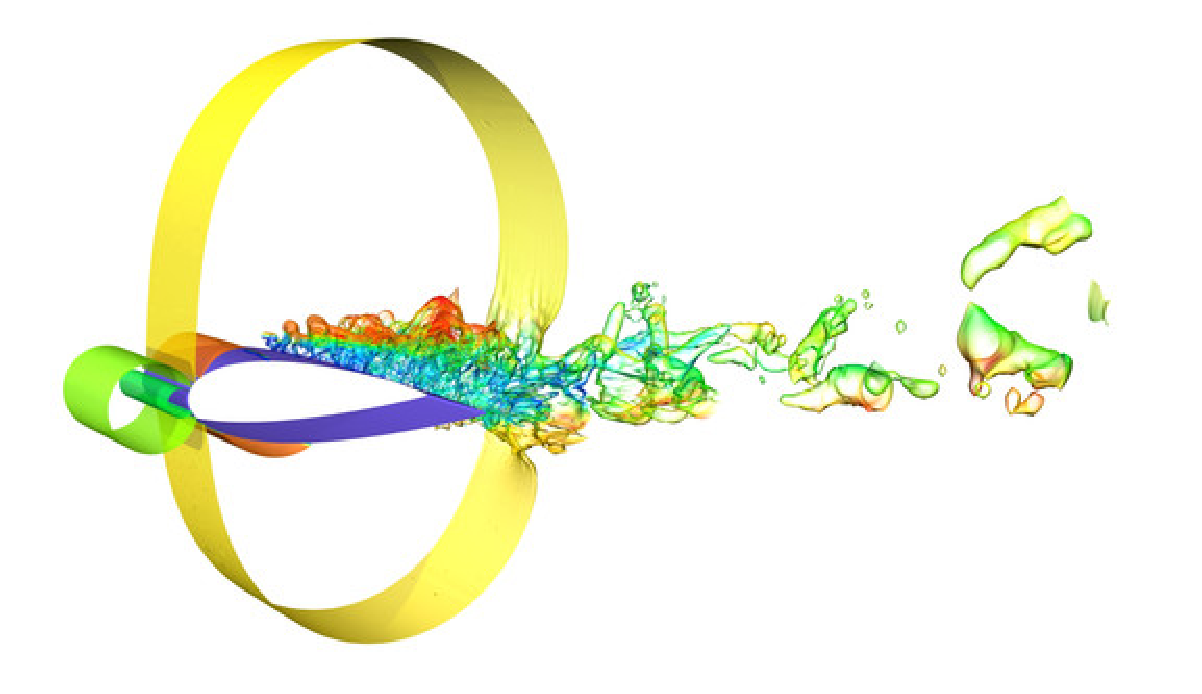
\includegraphics[width=0.6\textwidth]{./fig/example}
  \caption[Referenced name in the figure list]{Description of graphic below the figure.}
  \label{fig:GraphicLabel}
\end{figure}.

\subsubsection{Tables}
\label{sec:tab}

Similar to section \ref{sec:fig}, tables are to be included in a float
environment, namely \verb!table!, as follows:

\begin{verbatim}
  \begin{table}[placement specifier]
    \begin{tabular}{rcl}
      line 1 column 1 & column 2 $ column 3\\
      line 2 column 1 & column 2 $ column 3
    \end{tabular}
    \caption{Description of table.}
    \label{tab:TableName}
  \end{table}
\end{verbatim}

\verb!rcl! stands for \verb!right!, \verb!center!, and \verb!left! and
referres to the alignment of the column. "\verb!|!" inbetween will separate
the columns by a vertical line. \verb!\hline! after, e.g. \verb!\\! inserts a
horizontal line after the line (see also table \ref{tab:labelspec}
below). \LaTeX-tables are far from perfect if your table gets a bit more
complex, e.g. when inserting bigger equations. Formatting tables to someones
total satisfaction can be very tricky and trying to be too fancy is again
mostly a time waster. Keep it simple!

\subsection{Equations}
\label{sec:eq}

Equations with numbering should be included by the \verb!align! environment
like this
\begin{verbatim}
  \begin{align}\label{eq:EquationName}
    f(x) := \exp(x) &= \sum_{n=0}^{\infty} \frac{x^{n}}{n!} \nonumber \\
                    &\approx 1 + x + \frac{x^{2}}{2} + \frac{x^{3}}{6}
  \end{align}
\end{verbatim}
  or alternatively
\begin{verbatim}
  \begin{equation}\label{eq:EquationName}
   \begin{array}{rcl}
    f(x) := \exp(x) &= \sum_{n=0}^{\infty} \frac{x^{n}}{n!} \nonumber \\
                    &\approx 1 + x + \frac{x^{2}}{2} + \frac{x^{3}}{6}
   \end{array}
  \end{equation}
\end{verbatim}
for
~
\begin{align}\label{eq:EquationName}
  f(x) := \exp(x) &= \sum_{n=0}^{\infty} \frac{x^{n}}{n!} \nonumber \\
                  &\approx 1 + x + \frac{x^{2}}{2} + \frac{x^{3}}{6}.
\end{align}

Use \verb!\\! to insert a multiline equation. Use \verb!&! to align those 
to each other as shown. It defines one \verb!rl!-aligned pair, which means that
everything that stands on the left of \verb!&! will be right align and vice
versa.  The equation itself will be centered. Use \verb!\nonumber! to surpress
the numbering of certain lines as shown. If no numbering is wanted use
\verb!align*! and leave out the label. Look on the web for more complex
alignments - see also the \verb!alignat!-environment that could be used
alternatively. Use it scarcely. \verb!align! is powerfull and easy to use; it
should be used most (meaning 99\%) of the times.

Objects like vectors, matrices, and similar things should be formated
consistently using a dedicated command defined in the beginning of youe
\LaTeX-file. See for instance above the definition of \verb!\vec! for writing
a vector $\vec{x}$. Thus, you can also read your equations in \LaTeX-code more
easily. Additionally the nomenclature of an object is changed by
changing only one line in your header. 

It is recommended to insert sub- and superscript as well as any manipulation of
symbold like \verb!\hat! etc. by using \verb!{}! even when only one symbol is
manipulated, e.g. \verb!\hat{\vec{x}}_{i}! for $\hat{\vec{x}}_{i}$. It's good
coding and can otherwise also be an ever recurring source of typos and
compilation errors.
